\documentclass{article}

\usepackage[brazilian]{babel}
\usepackage{fancyhdr}
\usepackage{indentfirst}
%\usepackage{hyperref}
\usepackage{graphicx}
\usepackage{csquotes}
\MakeOuterQuote{"}

\pagestyle{fancy}
\pagestyle{empty}
\fancyhead{} % Clear the header
\fancyhead[C]{\hrulefill\ Introdução do Linux, Git e Python \hrulefill} 

\begin{document}

	\title{Introdução ao Linux, Git e programação em Python}
	\date{\today}
	\author{Omar Mesquita}
	\maketitle
	
	\newpage
	\tableofcontents
	\newpage

	\section{Linux}
	\subsection{Por que?}
	
	Para nosso projeto (e muitos outros em outros grupos de pesquisa, empresas, etc) será simplesmente mais conveniente 
	usar o Linux. Caso não tenha ouvido falar, o Linux, também chamado de GNU/Linux, é um sistema operacional, como o 
	Windows da Microsoft ou o macOS da Apple. 


	O que torna ele especial é o alto grau de \textit{liberdade} ofertado pela plataforma, o qual facilita muito a vida de nós, 
	desenvolvedores. Esse aspecto do sistema se expressa em várias características do Linux como o fato de ser código aberto. 
	No entanto, para fins desse livreto, ele se resume à agilidade e à eficiência de sua \textbf{linha de comando}.

	\subsection{Linha de comando? Aquele négocio de 1990?} 

	Resumidamente, sim. Agora, antes que isso pareça uma má ideia, posso garantir a você que uma vez entendida a essência da
	linha de comando e seus principais comandos, sua produtividade como pessoa desenvolvedora vai aumentar muito! 

	Conheço pessoas que já desenvolveram muito código (principalmente no Windows), 
	mas ficaram hesitantes quanto ao uso da CLI (sigla para interface de linha de comando, em inglês) 
	pela sua natureza um tanto "retrô" e por receio de não aprender todos os comandos, e,
	consequentemente, perder sua preciosa produtividade. 

	O lado bom é que ninguém sabe todos os comandos e realmente não é necessário. A \textbf{curva de aprendizado} pode, 
	inicialmente, parecer muito difícil de superar, mas não se iluda, você irá entender rapidinho. 

	Se familiarizar com a CLI, como qualquer processo de aprendizado, está sujeito ao \textit{Efeito Dunning Kruger}. 
	Inicialmente, você pode se desesperar achando que será algo difícil, tedioso ou demorado para dominar, mas assim que
	começar a praticar, as coisas vão ficando mais claras. 

	\begin{figure}[h!]
  		\centering
		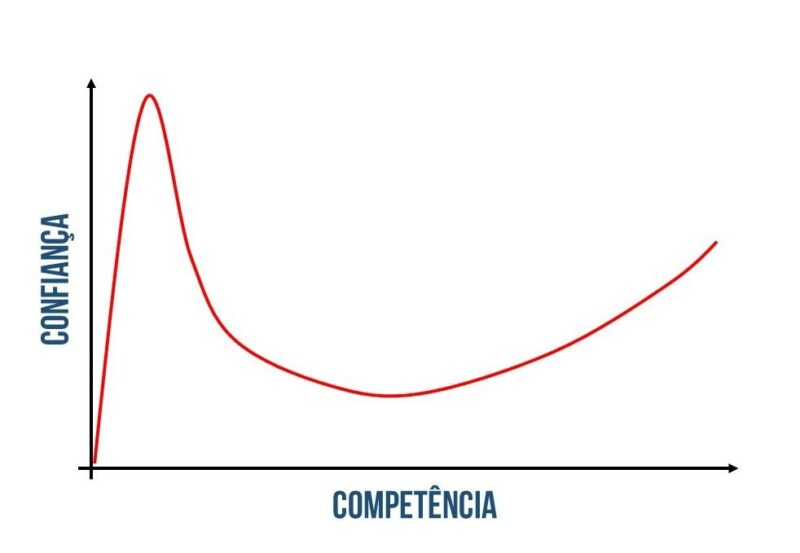
\includegraphics[scale=0.3]{figs/dk.jpeg} 
  		\caption{O efeito Dunning Kruger. Não deixe que o primeiro pico te desmotive!}
	\end{figure}
	
	Agora, podemos falar de comandos - vamos começar com os básicos, isto é, aqueles que você usa todo dia só que de forma gráfica
	em programas como o Explorador do Windows. Para digitar comandos, procuramos o aplicativo chamado \textbf{terminal} no 
	nosso sistema Linux. Ao clilcar nele, você irá se deparar com algo assim: 
	
	\vspace{1ex}
	\texttt{user@computador: ~}
	\vspace{1ex}

	O que significa que o usuário de nome \texttt{user} está, ou "at" em inglês, (\texttt{@}) no computador de nome
	\texttt{computador}. Depois dos dois pontos, irá aparecer os comandos que você digitar. Geralmente, a primeira coisa
	que se faz ao entrar no computador é saber onde você está. 
	
	\subsubsection{Onde estou? O pwd}
	Para descobrir sua localização no sistema de arquivos, digite \texttt{pwd} e pressione Enter. Esse comando vêm de 
	\textit{print working directory}, o que traduz, a grosso modo, para "mostre o diretório no qual se está trabalhando". O
	resultado esperado é um caminho ou \textit{path} como \texttt{/home/usuario}. 

	Isso indica que você está na pasta pessoal, ou "lar", do usuário de nome \texttt{usuario}. Essa pasta, por sua vez, está 
	na coleção de "lares" das pessoas que usam o sistema (\texttt{/home}). Por fim, essa coleção é só mais uma pasta no que 
	se chama de \textbf{raiz} do sistema de arquivos, representada por um \texttt{/}. 

	\subsubsection{O que eu tenho? O ls} 

	Agora que você sabe onde está, como descobrir o que tem em cada pasta? Para isso, use o comando \texttt{ls}. Isso deve
	retornar a lista de arquivos e pastas que estão dentro do diretório no qual está trabalhando. Por exemplo, em um sistema
	de uso pessoal, é esperado que \texttt{/home/usuario} tenha pastas como \texttt{Videos, Downloads, Imagens, Musica}, entre
	outras. 
	
	\subsubsection{Mudança de diretório. O cd} 

	Você também vai querer entrar e sair de demais pastas durante seu trabalho no computador. O comando de \textit{change
	directory}, \texttt{cd}, permite a navegação no sistema. Para acessar a pasta um nível acima da qual você está use 
	\texttt{cd ..} 


	Caso o diretório esteja na mesma pasta em que você se encontra, simplesmente adicione o nome desta depois do comando. 
	Por exemplo, \texttt{cd Videos} te leva aos seus vídeos. Você pode, também, ir para um \textit{local qualquer} no sistema
	de arquivos digitando seu \textit{path}. Para acessar uma pasta com programas instalados, use seu caminho em conjunto 
	com o comando: 
	
	\vspace{1ex}
	\texttt{cd /usr/bin} 
	\vspace{1ex}

	\subsubsection{Entrada e saída (I/O)}

	Aqui, trataremos de comandos que fazem \textit{writes}, ou "escritas", no disco do computador e, portanto, entram e saiem
	com bytes em disco. 

	\paragraph{Criação de arquivo:} 
	\paragraph{}
	Para gerar um arquivo de tipo qualquer, use o \texttt{touch}: 
	
	\begin{enumerate} 
		\item{Arquivo de texto: \texttt{touch Documentos/meuTexto.txt}} 
		\item{Arquivo de vídeo: \texttt{touch ../meuVideo.mp4}}
		\item{Arquivo de biblioteca: \texttt{touch /minhaBiblioteca.so}}
		\item{Arquivo qualquer: \texttt{touch arquivoGenerico}}
	\end{enumerate}

	\paragraph{Copiando arquivos:} 
	\paragraph{} 
	O comando \texttt{cp} permite que você copie arquivos de um lugar para outro. Vejamos seu uso: 
	\begin{enumerate} 
		\item{Copiando um arquivo: \texttt{cp Documentos/meuTexto.txt .}}
		\item{Copiando uma pasta: \texttt{cp -R Videos Documentos}}
	\end{enumerate} 


	Tá, temos coisas novas aqui. Primeiramente, repare que o comando toma dois parâmetros. O primeiro é 
	o \textit{o que será copiado}, enquanto que o segundo é \textit{para onde} o objeto será copiado. 
	
	Em segundo lugar, veja no caso 1 que copiei o arquivo de texto \texttt{meuTexto.txt} da pasta \texttt{Documentos} 
	para o diretório no qual \textit{atualmente estou}. Se lembra que \texttt{..} representa a pasta um nível acima
	na hierarquia? Então, um ponto sozinho simboliza a pasta na qual você está trabalhando. 
	
	Por fim, para copiar uma pasta passamos uma \textbf{flag} para \texttt{cp} junto de seus argumentos. 
	A \textit{flag} \texttt{-R} funciona como um modificador do comando e, nesse caso, manda o \texttt{cp}
	copiar \textbf{recursivamente} o arquivo especificado, ou seja, o comando "entra" na pasta e copia o que
	tem dentro dela, \textbf{incluindo} a própria pasta. 

	
	\paragraph{Movendo arquivos}
	\paragraph{}

	Mover arquivos funciona de forma análaga ao \texttt{cp}, com uma diferença significativa sendo que não é necessário 
	especificar a flag \texttt{-R} para mover pastas - basta usar o comando como se fossem arquivos ordinários. 

	\begin{enumerate} 
		\item{\texttt{mv Documentos DocumentosSecretos}} 
		\item{\texttt{mv Videos/meuVideo.mp4 Downloads}} 
		\item{\texttt{mv meuTexto.txt Downloads/curriculo.txt}} 
	\end{enumerate} 


\end{document}

%\section{Git}
%\section{Python}

